\documentclass[a4paper,graphics,11pt,notitlepage]{scrartcl}

\usepackage{graphicx,curves,epsf,float,rotating}
\usepackage{epsf,epsfig,eepic}
\usepackage{latexsym,amsmath,amssymb}
\usepackage{amsmath}
\usepackage[utf8]{inputenc}
\usepackage{theorerms}
\usepackage{dcolumn}
\usepackage{tikz}
\usepackage{pgfplots}
\usepackage{enumerate}
\usepackage{footnote}
%\usepackage{biblatex}
\usepackage{fancyhdr}
\usepackage[english]{babel}

\usepackage[
colorlinks=false,
bookmarksnumbered = true,
linkbordercolor= white,
citebordercolor= white,
urlbordercolor= white]{hyperref}



%\textwidth 15cm
%\textheight 23cm
%\oddsidemargin 1cm
%\evensidemargin 0cm
%\parindent 0mm

\title{Solutions to Sheet 1}
\author{Friedrich May, 355487; Mariem Mounir}

\begin{document}
  \vspace{-5ex}
  \maketitle
  \section*{Exercise 1}
  \begin{tabular}{l|c|c|c|c}
    Norm&\multicolumn{2}{c}{Euclidian}&\multicolumn{2}{c}{Manhattan}\\\hline
    k&2&3&2&3\\\hline
    4,3,3&1&1&1&1\\
    4,-1,1&tie&-1&tie&1\\
    -2,4,5&-1&-1&tie&1\\
    -2,-6,1&tie&1&tie&1\\
    6,0,2&tie&1&-1&-1
  \end{tabular}
\section*{Exercise2}
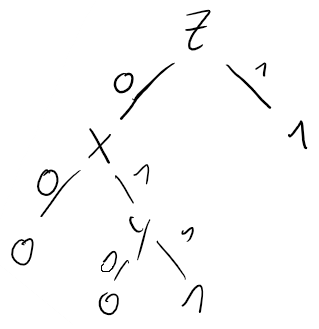
\includegraphics[scale=0.5]{E2Tree.png}
The first split is done using $z$, because this is the only variable for wich the result stays the same for a value of the variable.
The other two splits could be swapped because the influence on the result is the same for both variables.
\end{document}